\documentclass[12pt,a4paper,oneside]{book}
\usepackage[utf8]{inputenc}
\usepackage{graphicx} %input gambar
\usepackage{amsmath}
\usepackage{amsfonts}
\usepackage{amssymb}
\usepackage{float}
%Mengatur ke font times new rouman
\usepackage{mathptmx}

\usepackage[T1]{fontenc}
%
\usepackage{pdfpages}

% Garis tepi (margin)
%\usepackage[paperheight=29.7cm,paperwidth=21cm]{geometry}
\usepackage{geometry}
 \geometry{
 left=4cm,
 top=4cm,
 right=3cm,
 bottom=3cm,
 }

% mengatur 1 cm baris pertama paragraf
\usepackage{indentfirst}
\setlength{\parindent}{1cm}

% Mengkompres cite
\usepackage[numbers]{natbib}

% Mengatur page number
\usepackage{fancyhdr}
\pagestyle{fancy}
\renewcommand{\headrulewidth}{0pt} %menghilangkan garis

% change name Daftar Isi, Daftar Pustaka jadi section
\renewcommand{\contentsname}{DAFTAR ISI}
\renewcommand{\chaptername}{BAB}
\renewcommand{\bibname}{DAFTAR PUSTAKA}
\renewcommand{\listfigurename}{DAFTAR GAMBAR}
\renewcommand{\figurename}{Gambar}
\renewcommand{\listtablename}{DAFTAR TABEL}
\renewcommand{\tablename}{Tabel}
\renewcommand{\appendixname}{Lampiran}

% change languange dan pemenggalan kata
%\usepackage[indonesian]{babel}
\sloppy %agar teks tidak lebih saat rata kanan kiri

% numbering
\renewcommand{\thechapter}{\Roman{chapter}} %Peringkat 1
\renewcommand{\thesection}{\Alph{section}.} %Peringkat 2
\renewcommand{\thesubsection}{\arabic{subsection}.} %Peringkat 3
\renewcommand{\thefigure}{\arabic{chapter}.\arabic{figure}}%gambar
\renewcommand{\thetable}{\arabic{chapter}.\arabic{table}}%tabel
\renewcommand{\theequation}{\arabic{chapter}.\arabic{equation}}%equestion

\setcounter{secnumdepth}{3}
\renewcommand{\thesubsubsection}{\thesubsection\arabic{subsubsection}}

% baris antar paragraf
\linespread{1.5}

% mengatur title section
\usepackage{titlesec}
\titleformat{\chapter}[display]   
{\centering\normalfont\large\bfseries}
{\MakeUppercase{\chaptertitlename}\ \thechapter}{0pt}{\large}   
\titlespacing*{\chapter}{0pt}{-50pt}{40pt}
% ukuran section dan subsection
\titleformat{\section}
  {\normalfont\fontsize{12}{15}\bfseries}{\thesection}{1em}{}
\titleformat{\subsection}
  {\normalfont\fontsize{12}{15}\bfseries}{\thesubsection}{1em}{}

% untuk modif numbering
\usepackage{enumitem}

% membuat link
\usepackage{hyperref}

%\usepackage{soul} %digunakan sementara untuk meng-highlight teks yang belum diubah

\usepackage[none]{hyphenat} %untuk menghilangkanpemenggalan kata

% Perlengkapan pada table
\usepackage{colortbl} %untuk color table
\usepackage{adjustbox} %agar table pas di halaman (tidak lebih)
\usepackage{longtable} %Untuk membuat table lebih panjang
\usepackage{multirow}

\usepackage{float} %digunakan agar gambar dan tabel tidak pindah, cara menggunakan dengan menambah [H]

% Untuk membuat flowchart
\usepackage{tikz}
\usetikzlibrary{shapes.geometric, arrows}

\usepackage{wrapfig} %untuk menambah wrap figure

% Untuk membuat subfigure, dan subtable
\usepackage[labelsep=space,labelfont=bf,font=bf]{caption} %menghilangkan titik dua (:), tebal pada caption gambar
\usepackage{subcaption}

\begin{document}

\newpage
\begin{titlepage}
   \begin{center}

       \textbf{PENERAPAN $K$-MEANS DAN ALGORITMA GENETIKA UNTUK MENYELESAIKAN MTSP}
       
       (Studi Kasus Pada Perjalanan Menuju Seluruh SMA di Kabupaten Probolinggo)

       \vfill
       \textbf{SKRIPSI}
       \vfill
       
       
\includegraphics[width=0.4\textwidth]{Gambar/logo.png}
       
       \vfill
       
       \textbf{OLEH:}\\
       \textbf{\underline{MUHAMMAD FAIZ NAILUN NI'AM}}\\
       NIM : 1842200034

       \vfill
       
       UNIVERSITAS NURUL JADID\\
       PAITON PROBOLINGGO\\
       \textbf{FAKULTAS SOSIAL DAN HUMANIORA}\\       
       PROGRAM STUDI PENDIDIKAN MATEMATIKA\\
       
       \vfill       
       
       AGUSTUS 2022
       
   \end{center}
\end{titlepage}

% Halaman depan
\newpage
\frontmatter
\begin{center}

\textbf{PENERAPAN $K$-MEANS DAN ALGORITMA GENETIKA UNTUK MENYELESAIKAN MTSP}
       
       (Studi Kasus Pada Perjalanan Menuju Seluruh SMA di Kabupaten Probolinggo) 
       
       \vfill
       \textbf{SKRIPSI}
       \vfill
       
       DIAJUKAN KEPADA UNIVERSITAS NURUL JADID \\
       PAITON PROBOLINGGO UNTUK MENYELESAIKAN \\ SALAH SATU PERSYARATAN DALAM MENYELESAIKAN \\ PROGRAM SARJANA PENDIDIKAN MATEMATIKA
       
       \vfill       
       
       \textbf{OLEH :}\\
       \textbf{\underline{MUHAMMAD FAIZ NAILUN NI'AM}}\\
       NIM : 1842200034

       \vfill
       
       UNIVERSITAS NURUL JADID\\
       PAITON PROBOLINGGO\\
     \textbf{FAKULTAS SOSIAL DAN HUMANIORA}\\       
       PROGRAM STUDI PENDIDIKAN MATEMATIKA\\
       
       \vfill       
       
       JULI 2022
       
   \end{center}

%\newpage
%\addcontentsline{toc}{chapter}{PERSETUJUAN PEMBIMBING SKRIPSI}
%\includepdf[pages={2}]{lembar persetujuan pembimbing.pdf}

%\newpage
%\addcontentsline{toc}{chapter}{PENGESAHAN TIM PENGUJI SKRIPSI}
%\includepdf[pages={2}]{lembar persetujuan dan pengesahan.pdf}

%\newpage
%\addcontentsline{toc}{chapter}{PERNYATAAN KEASLIAN TULISAN}
%\includepdf[pages={2}]{pernyataan keaslian tulisan bermaterai.pdf} ...

\newpage
\chapter*{ABSTRAK}

Beberapa lembaga pendidikan sering kali mengadakan acara-acara besar seperti kompetisi dan olimpiade. Permasalahan pendistribusian barang  seperti poster, surat selebaran, dan undangan seringkali terjadi keterlambatan. Bagaimana menentukan rute optimum bagi beberapa pengirim barang di sebuah lembaga pendidikan akan dimodelkan secara matematis dan akan diselesaikan menggunakan metode $k$-means dan algoritma genetika. Permasalahan ini termasuk kategori \textit{Multiple Travelling Salesman Problem}. Dalam skripsi ini dilakukan pencarian rute optimum untuk menuju seluruh SMA di Kabupaten Probolinggo menggunakan $k$-means dan algoritma genetika.

\vspace{0.5cm}

\noindent \textbf{Kata Kunci:} MTSP, Algoritma Genetika, $K$-means.

\chapter*{ABSTRACT}

Some educational institutions often hold big events such as competitions and Olympics. Problems with the distribution of goods such as posters, leaflets, and invitations often result in delays. How to determine the optimum route for several shippers in an educational institution will be modeled mathematically and will be solved using the $k$-means method and genetic algorithm. This problem belongs to the \textit{Multiple Traveling Salesman Problem} category. In this thesis, the search for the optimum route to all high schools in Probolinggo Regency is conducted using $k$-means and genetic algorithms.

\vspace{0.5cm}

\noindent \textbf{Kata Kunci:} MTSP, Genetic Algorithms, $K$-means.
\newpage
\chapter*{KATA PENGANTAR}

Segenap puji dan syukur kami panjatkan kepada Tuhan Yang Maha Esa karena atas berkat, karunia, dan rahmat yang diberikan oleh-Nya, sehingga penulis berkesempatan untuk menyelesaikan penelitian skripsi ini yang berjudul "Penerapan $K$-means dan Algoritma Genetika untuk Menyelesaikan MTSP (Studi Kasus pada Perjalanan Menuju Seluruh SMA di Kabupaten Probolinggo)".

Dalam penelitian dan penyusunan laporan ini, telah mendapatkan banyak bantuan, dukungan, bimbingan, serta do'a yang sangat berharga sehingga penulisan skripsi ini dapat berjalan sesuai dengan waktu yang telah ditentukan.
Oleh karena itu kami ingin mengucapkan terima kasih yang sebesar-besarnya kepada pihak yang telah memberikan dukungan dan membantu selama penyusunan skripsi ini.

\begin{enumerate}
	\item Keluarga terutama orang tua yang telah memberikan semangat dan motivasi dalam menyelesaikan penelitian ini.
	\item Bapak \hl{[[nama bapak hamid]]} dan Ibu \hl{[[nama ibu shofia]]} selaku dosen pembimbing yang telah meluangkan waktu dan tenaganya serta memberikan bimbingan, wawasan, dan ilmu yang sangat berharga dalam menyelesaikan penelitian ini.
	\item Ibu \hl{[[nama bu olief]]} selaku dosen penguji proposal yang telah memberikan masukan, nasehat, dan perbaikan pada proposal penelitian yang sebelumnya telah dibuat.
	\item Seluruh teman-teman dari Prodi Matematika angkatan 2018 sebagai teman seperjuangan dalam menyelesaikan skripsi yang juga saling memberikan semangat dan dukungan dalam menyelesaikan skripsi.
	\item Semua pihak yang secara langsung maupun tidak langsung terlibat dalam membantu penulis menyelesaikan skripsi ini.
\end{enumerate}

Kami menyadari bahwa dalam penelitian ini masih terdapat kekurangan dan jauh dari kata sempurna. Oleh karena itu kami menerima dengan baik segala kritik dan masukan yang dapat membangun bagi kami. Kami berharap skripsi ini dapat memberi manfaat bagi banyak pihak.

\begin{flushright}
Probolinggo, 26 Mei 2022\\
Penulis
\end{flushright}

\newpage
%\addcontentsline{toc}{chapter}{DAFTAR ISI}
\tableofcontents

\newpage
%\addcontentsline{toc}{chapter}{DAFTAR GAMBAR}
\listoffigures

%\newpage
%\listoftables

% Halaman utama
\newpage
\mainmatter

\chapter{PENDAHULUAN}

\section{Latar Belakang Masalah}

Kabupaten Probobolinggo adalah salah satu dari beberapa kabupaten yang sedang berkembang di provinsi Jawa Timur. Banyak sekolah tingkat menengah yang tersebar di Kabupaten Probolinggo. Selain itu di Kabupaten Probolinggo terdapat beberapa kampus di dalamnya, salah satunya adalah Universitas Nurul Jadid yang terletak di Kecamatan Paiton. Pada tahun-tahun sebelumnya kampus ini sering sekali mengadakan acara-acara besar seperti olimpiade. Dalam acara-acara seringkali melakukan pendistribusian barang seperti undangan acara, pamflet, dan lain-lain kepada sekolah-sekolah di Kabupaten Probolinggo. Oleh karena itu diperlukanlah sebuah pencarian rute yang efisien untuk menuju ke sekolah-sekolah tersebut agar dapat menghemat waktu dan tenaga dalam perjalanan. Permasalahan pencarian rute tersebut dalam hal ini dapat disebut dengan \textit{Traveling Salesman Problem}. Sedangkan gabungan dari beberapa permasalahan TSP biasa disebut \textit{Multiple Traveling Salesman Problem} (MTSP).

Selama bertahun-tahun, telah banyak penelitian tentang \textit{Multiple Traveling Salesman Problem} (MTSP). Berbagai metode telah banyak digunakan untuk mencari solusi MTSP salah satunya adalah Algoritma Genetika (AG) dan Ant Colony. Tahap pertama dalam MTSP adalah pengklasteran (pengelompokan data) sebelum melakukan pencarian solusi, ada banyak cara untuk menggunakan AG dalam pengklasteran, terbukti bahwa metode ini dapat mengklaster data lebih cepat daripada beberapa algoritma lain yang digunakan untuk pengklasteran \cite{krishna1999genetic}. Kemampuan pengklasteran dari AG ini dimanfaatkan untuk mencari pusat klaster yang sesuai sehingga kesamaan dari klaster yang dihasilkan dioptimalkan \cite{maii2000genetic}. Ada juga upaya untuk menggunakan metode paralel untuk TSP untuk meningkatkan efisiensi \cite{li2016parallel}.

Namun, menurut artikel Zhang efisiensi AG akan menurun dengan cepat jika digunakan pada skala kota besar \cite{zhang2014parallel}, berbeda dengan algoritma $k$-means dapat mengklaster dan menghindari persilangan tiap rute salesman (pengantar barang) \cite{inproceedings}. Penggunaan Algoritma Genetika dan dan algoritma \textit{k}-means adalah metode yang efektif untuk menyelesaikan MTSP, selain itu juga dapat menghindari persilangan rute antar salesman seperti yang dibahas oleh Lu pada artikelnya \cite{inproceedings}. Dari gabungan semua perspektif tersebut, dalam penelitian ini, digunakanlah \textit{k}-means dan Algoritma Genetika untuk menyelesaikan kasus pembagian klaster dan pencarian rute terdekat menuju seluruh SMA di Kabupaten Probolinggo.
%\section{Identifikasi Masalah}

Dari latar belakang yang telah diuraikan,
identifikasi masalahnya adalah sebagai berikut.
\begin{enumerate}
	\item Penggunaan $k$-means dan algoritma genetika untuk mencari solusi MTSP.
	\item Pembagian klaster dan rute terdekat tiap klaster seluruh SMP yang ada di Kabupaten Probolinggo.
\end{enumerate}
\section{Rumusan Masalah}

Berdasarkan identifikasi masalah, maka rumusan masalah yang akan dikaji dalam penelitian ini sebagai berikut:
\begin{enumerate}
    \item Bagaimana cara mencari solusi \textit{multiple traveling salesman problem} dengan $k$-means dan algoritma genetika?
    \item Bagaimana pembagian klaster dan penentuan rute terdekat menuju seluruh SMA di Kabupaten Probolinggo?
\end{enumerate}
\section{Tujuan Penelitian dan Pengembangan}

Berdasarkan rumusan masalah, tujuan dari penelitian ini yaitu untuk:
\begin{enumerate}
	\item Mengetahui cara menemukan solusi \textit{multiple traveling salesman problem} dengan $k$-means dan algoritma genetika.
	\item Menemukan solusi pembagian klaster dan penentuan rute terdekat menuju seluruh SMA di Kabupaten Probolinggo.
\end{enumerate}

% sudah direvisi ibu shofia

\section{Manfaat Penelitian}

Manfaat dari penelitian ini yaitu:
\begin{enumerate}
	\item Bagi Penulis, mengetahui cara menyelesaikan kasus permasalahan \textit{Multiple Traveling Salesman Problem} yang telah dipelajari yaitu dengan menggunakan metode $K$-Means \textit{Clustering} dan Algoritma Genetika serta penulis dapat mengembangkan ilmu pemrograman python pada komputer.

	\item Bagi Program Studi Pendidikan Matematika, menambah ilmu mengenai metode optimasi dan pencarian rute terdekat yang dapat diterapkan serta dipelajari kembali oleh mahasiswa pendidikan matematika untuk tahun-tahun selanjutnya, serta mengetahui rute-rute terdekat untuk menuju ke seluruh SMA di Kabupaten Probolinggo.
	
	\item Bagi Masyarakat, dapat menggunakan metode tersebut untuk menyelesaikan kasus \textit{Multiple Traveling Salesman Problem}, seperti penyebaran pestisida, pengintaian musuh pada militer, pendistribusian barang, dan lain-lain.
	
\end{enumerate}
\section{Batasan Masalah Penelitian}

Berdasarkan latar belakang penelitian dan tujuan penelitian, batasan masalah dalam penelitian ini yaitu:

\begin{enumerate}
	\item MTSP pada skripsi ini menggunakan 1 kota asal dan setiap salesman akan berangkat dan kembali pada simpul kota yang sama.
	\item MTSP pada skripsi ini menggunakan menggunakan $k$-means untuk pengklasteran dan algoritma genetika untuk menentukan rute terdekatnya.
	\item Banyak titik tujuan selalu lebih besar dari setiap salesman.
	\item Titik tujuan merupakan SMA di seluruh Kabupaten Probolinggo baik negeri maupun swasta.
	\item Setiap titik tujuan diasumsikan selalu terhubung dan berjalan lurus
	\item Tidak ada prioritas kota mana saja yang dilalui terlebih dahulu
\end{enumerate}
%\section{Definisi Konsep}

Dalam proposal ini, membahas tentang \textit{Multiple Traveling Salesman Problem} yang merupakan perluasan dari \textit{Travelling Salesman Problem} (TSP). TSP adalah permasalahan pencarian rute terpendek seorang \textit{salesman} dari suatu kota ke kota lain tepat satu kali dan kembali ke kota yang sama. Sedangkan MTSP adalah permasalahan TSP oleh beberapa orang \textit{salesman} dengan tujuan yang sudah dibagi.

Algoritma yang digunakan untuk membagi adalah $K$-means. $K$-means adalah jenis metode klasifikasi yang membagi item data menjadi beberapa klaster. Algoritma Genetika (AG) digunakan untuk pencarian rute terpendek. AG adalah algoritma yang digunakan untuk mencari solusi dari permasalahan dengan cara yang terispirasi dari teori evolusi. Dalam hal ini, algoritma genetika dapat juga digunakan untuk pencarian sebuah rute terpendek dalam sebuah kasus perjalanan. Untuk mengukur jarak antar 2 titik yang digunakan adalah metode \textit{euclidean distance}.


\chapter{KAJIAN PUSTAKA}
% sudah direvisi ibu shofia

\section{Penelitian Relevan}

Ada beberapa hasil penelitian sebelumnya yang memiliki keterkaitan dengan penelitian ini. Penelitian berjudul "Applying K-means and Genetic Algorithm for Solving MTSP" \cite{inproceedings}. Penelitian tersebut membahas tentang persilangan jalur antar tiap salesman yang dapat dihindari dengan menggukan Algoritma Genetika dan \textit{K}-means.

Penelitian kedua berjudul "Optimasi \textit{Multiple Travelling Salesman Problem} (M-TSP) Pada Penentuan Rute Optimal Penjemputan Penumpang \textit{Travel} Menggunakan Algoritme Genetika" \cite{raditya2017optimasi}. Penelitian tersebut membahas tentang permasalahan MTSP yaitu beberapa orang salesman yang akan berangkat dari kantor \textit{travel} menuju ke alamat penjemputan masing-masing penumpang. Pada permasalahan tersebut menggunakan representasi permutasi, proses reproduksi \textit{crossover} dengan \textit{one cut point crossover}, proses mutasi dengan \textit{exchange mutation}, dan proses seleksi dengan \textit{elitism selection}.

Mayuliana, N. K., Kencana, E. N., dan Harini, L. P. I. dalam artikelnya yang berjudul “Penyelesaian Multitraveling Salesman Problem dengan Algoritma Genetika” \cite{mayuliana2015penyelesaian}, mempelajari tentang kinerja algoritma genetika berdasarkan jarak minimum dan waktu pemrosesan yang diperlukan untuk 10 kali pengulangan untuk setiap kombinasi kota penjual. Artikel karangan Al-Khateeb, B., dan Yousif, M. berjudul "\textit{SOLVING MULTIPLE TRAVELING SALESMAN PROBLEM BY MEERKAT SWARM OPTIMIZATION ALGORITHM}" \cite{al2019solving} dalam artikel ini mengusulkan algoritma metaheuristik yang disebut algoritma \textit{Meerkat Swarm Optimization} (MSO) untuk memecahkan MTSP dan menjamin solusi berkualitas baik dalam waktu yang wajar untuk masalah kehidupan nyata.

\section{Dasar Teori}

\chapter{KERANGKA TEORITIK DAN PENGEMBANGAN}
%model penelitian dan pengembangan
%prosedur penelitian dan pengembangan
\section{Metode Penelitian}

Metode penelitian dalam proposal ini adalah metode penelitian dan pengembangan. Melalui metode ini diharapkan dapat mengembangkan algoritma yang diteliti.

\subsection{Data Dalam Penelitian}
    
Data yang digunakan dalam penelitian ini adalah data koordinat dari seluruh SMP yang ada di Kabupaten Probolinggo. Data dikumpulkan dari \url{https://data.sekolah-kita.net}. Waktu yang diperlukan peneliti untuk mengumpulkan data dari web tersebut adalah 1 bulan karena data dikumpulkan secara manual.

\subsection{Instrumen Pendukung}
\begin{enumerate}
    \item Python
    
    Dalam penelitian ini akan digunakan bahasa pemrograman python untuk mempermudah pengerjaan. Bahasa python adalah bahasa pemrograman baru di masa sekarang, karena dalam bahasa ini lebih simple dan singkat dalam membuat program \cite{syahrudin2018input}. Bahasa pemrograman ini merupakan bahasa pemrograman yang paling mudah dipelajari dari pada bahasa pemrograman yang lain.
    
    \item Jupyter Notebook
    
    Jupyter Notebook adalah aplikasi web gratis yang digunakan untuk membuat dan membagikan dokumen yang memiliki kode, hasil hitungan, visualisasi, dan teks. Notebook ini juga mendukung 3 bahasa pemrograman salah satunya adalah bahasa pemrograman python.

	\item Google Earth
	
	Google earth digunakan dalam penelitian ini untuk mengumpulkan koordinat lokasi seluruh SMP yang ada di Kabupaten Probolinggo. Dalam hal ini google earth dapat menandai beberapa lokasi dan mengexport langsung kedalam bentuk excel. Data-data lokasi yang telah didownload ke dalam bentuk excel akan diproses menggunakan jupyter notebook.

\end{enumerate}

\subsection{Langkah-langkah Dalam Penelitian}
\begin{enumerate}
    \item Menyiapkan dataset yang telah dikumpulkan sebelumnya.
    \item Selanjutnya menentukan jumlah klaster yaitu sebanyak $n$ klaster. Data yang telah dikumupulkan pada tahap ini akan dibagi menjadi beberapa klaster, metode yang digunakan algoritma \textit{k}-means.
    \item Langkah-langkah yang digunakan dalam metode \textit{k}-means adalah sebagai berikut
    \begin{enumerate}
        \item Memilih sebanyak $n$ \textit{centroid} secara acak, sesuai dengan berapa banyak salesman yang akan ditugaskan
        \item Menghitung jarak data ke \textit{centroid} dengan rumus \textit{euclidean distance}
        \begin{equation}
        d_{xy}=\sqrt{\sum_{i=1}^{n}(x_i-y_i)^{2}}
        \end{equation}
        \item Titik-titik lokasi yang tersebar merupakan klaster yang sama dengan titik \textit{centroid} paling dekat
        \item Perbarui \textit{centroid} tiap klaster yang dihasilkan dengan menghitung nilai koordinat rata-rata titik nilai pada masing-masing klaster.
        \item Iterasi dilakukan untuk generasi berikutnya sampai yaitu dengan kembali ke tahapan (b) sampai tidak ada perubahan klaster atau perubahan nilai \textit{centroid}
    \end{enumerate}
	
	\item Selanjutnya melakukan proses TSP pada setiap klaster yang telah dibagi, langkah-langkahnya adalah sebagai berikut.
	\begin{enumerate}
	    \item Membuat populasi awal secara random menggunakan data yang telah diklaster
	    \item Melakukan reproduksi dengan metode \textit{crosover} dengan peluang 0,95
	    \item Melakukan mutasi pada data dengan peluang 0,01
	    \item Selanjutnya seleksi dengan mode eliminasi
	    \item Menentukan nilai fitness agar mendapatkan solusi akhir yang optimaldengan rumus:
	    \begin{equation}
	    fitness=\frac{10000}{RMSE}
	    \end{equation}
	    \item Iterasi dilakukan dengan cara kembali ke tahapan b untuk generasi berikutnya sampai hasil yang dilakukan optimal atau mendekati optimal.
    \end{enumerate}
	\item Ketika proses diatas selesai dilakukan maka dihasilkanlah pembagian klaster dan rute terdekat tiap klaster menuju seluruh SMP di Kabupaten Probolinggo
	\item Menganalisa dan mengevaluasi data yang dihasilkan
\end{enumerate}

\section{Prosedur Penelitian dan Pengembangan}


\subsection{Data Penelitian}
    
Berdasarkan studi kasus dalam skripsi ini, data yang akan digunakan dalam penelitian ini adalah data koordinat dari seluruh SMA di Kabupaten Probolinggo. Data nama-nama sekolah dikumpulkan dari \url{https://data.sekolah-kita.net}, dan data koordinat dikumpulkan melalui aplikasi Google Earth yang dapat diunduh langsug ke dalam bentuk excel. Waktu yang diperlukan peneliti untuk mengumpulkan data dari web tersebut kurang lebih sekitar satu bulan.

\subsection{Instrumen Pendukung}
\begin{enumerate}
    \item Python
    
    Dalam penelitian ini akan digunakan bahasa pemrograman python untuk mempermudah pengerjaan. Bahasa python adalah bahasa pemrograman baru di masa sekarang, karena dalam bahasa ini lebih simple dan singkat dalam membuat program \cite{syahrudin2018input}. Bahasa pemrograman ini merupakan bahasa pemrograman yang paling mudah dipelajari dari pada bahasa pemrograman yang lain. Serta dalam bahasa pemrograman ini dapat menjalankan beberapa rumus matematika di dalamnya.
    
    \item Jupyter Notebook
    
    Jupyter Notebook adalah aplikasi web gratis yang digunakan untuk membuat dan membagikan dokumen yang memiliki kode, hasil hitungan, visualisasi, dan teks. Notebook ini juga mendukung 3 bahasa pemrograman salah satunya adalah bahasa pemrograman python. Banyak kelebihan yang disajikan dari aplikasi ini salah satunya adalah visualisasi data, mendokumentasikan kode, dan menjalankan kode dalam setiap sel.

\begin{figure}[h!]
  \centering
  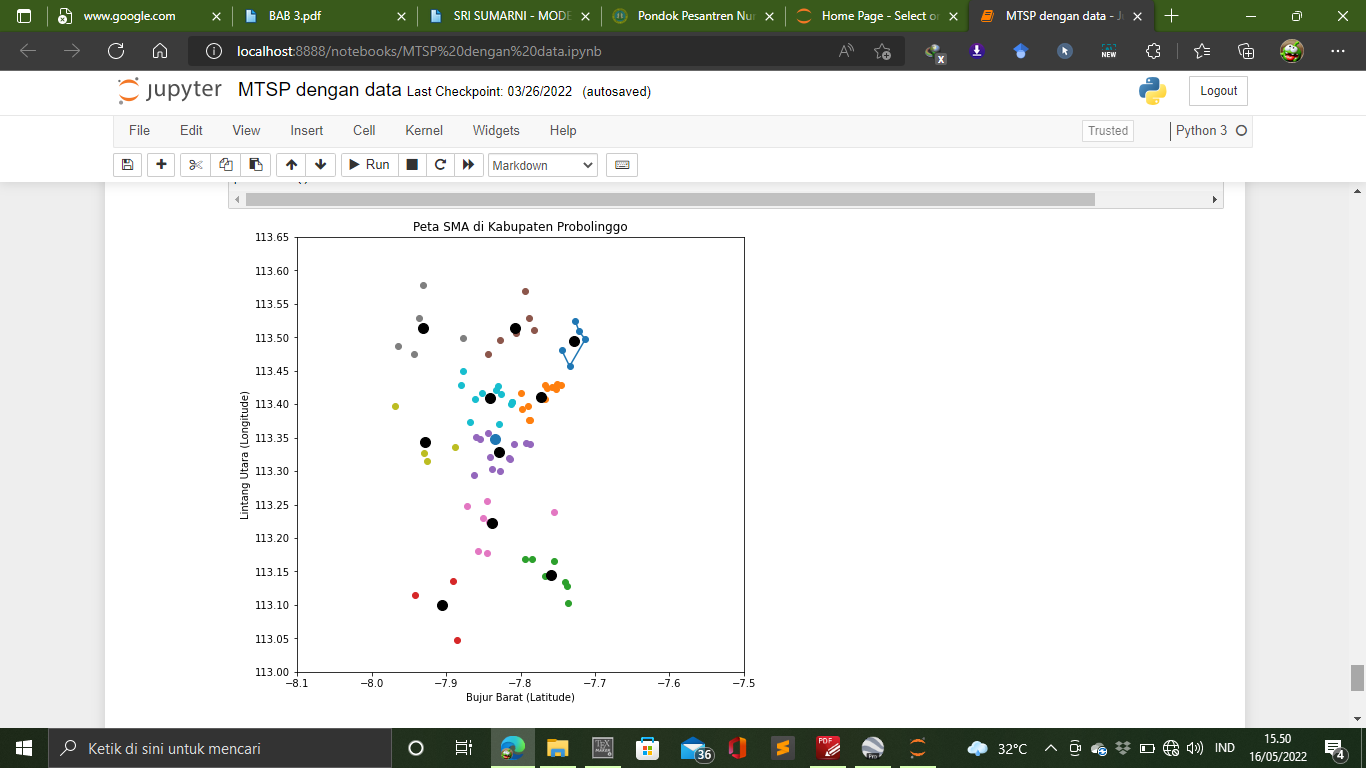
\includegraphics[width=0.8\textwidth]{visualisasi jupyter.png}
  \caption{Visualisasi data menggunakan jupyter notebook}
\end{figure}

	\item Google Earth
	
	Google earth digunakan dalam penelitian ini untuk mengumpulkan koordinat lokasi seluruh SMA di Kabupaten Probolinggo. Dalam hal ini google earth dapat menandai beberapa lokasi dan mengekspor langsung kedalam bentuk excel. Data-data lokasi yang telah didownload ke dalam bentuk excel akan diproses menggunakan jupyter notebook.

\begin{figure}[h!]
  \centering
  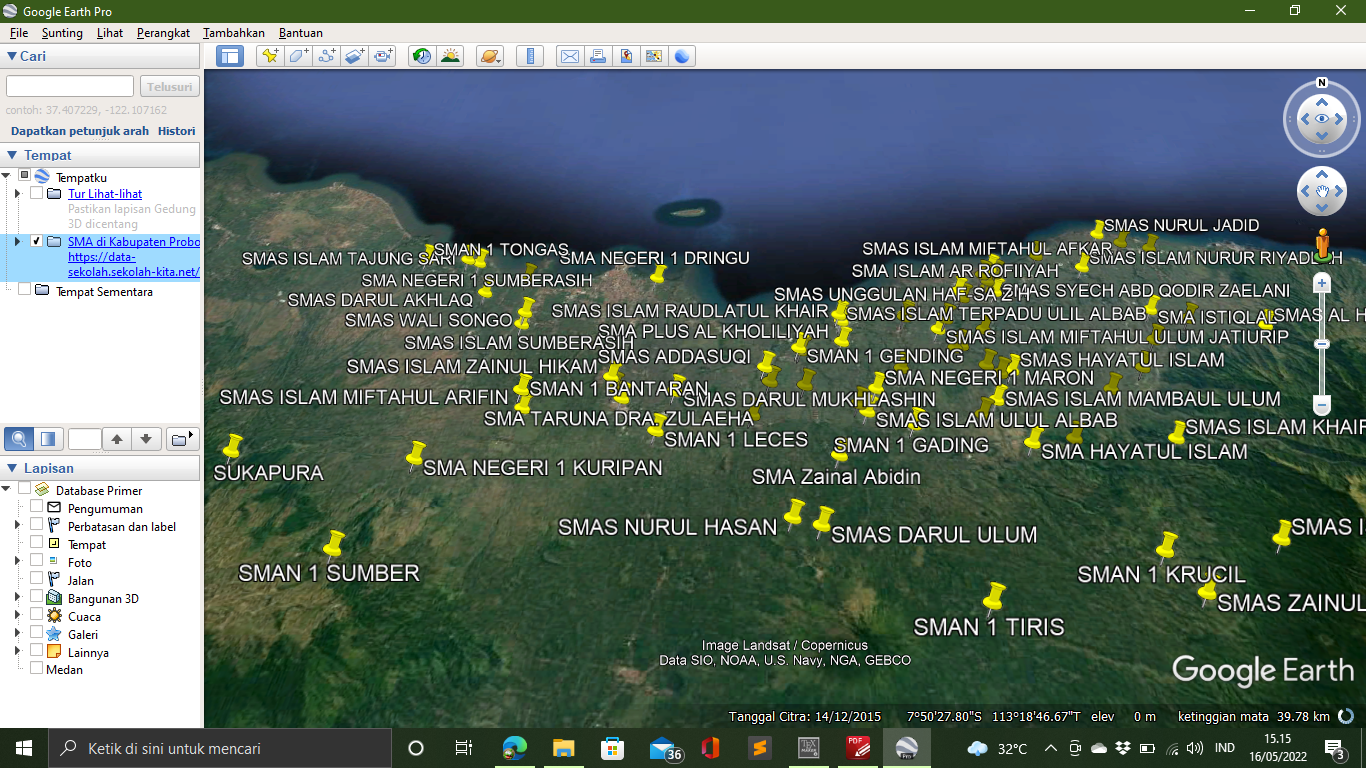
\includegraphics[width=0.8\textwidth]{google earth.png}
  \caption{Menandai beberapa lokasi pada google earth}
\end{figure}

\begin{figure}[h!]
  \centering
  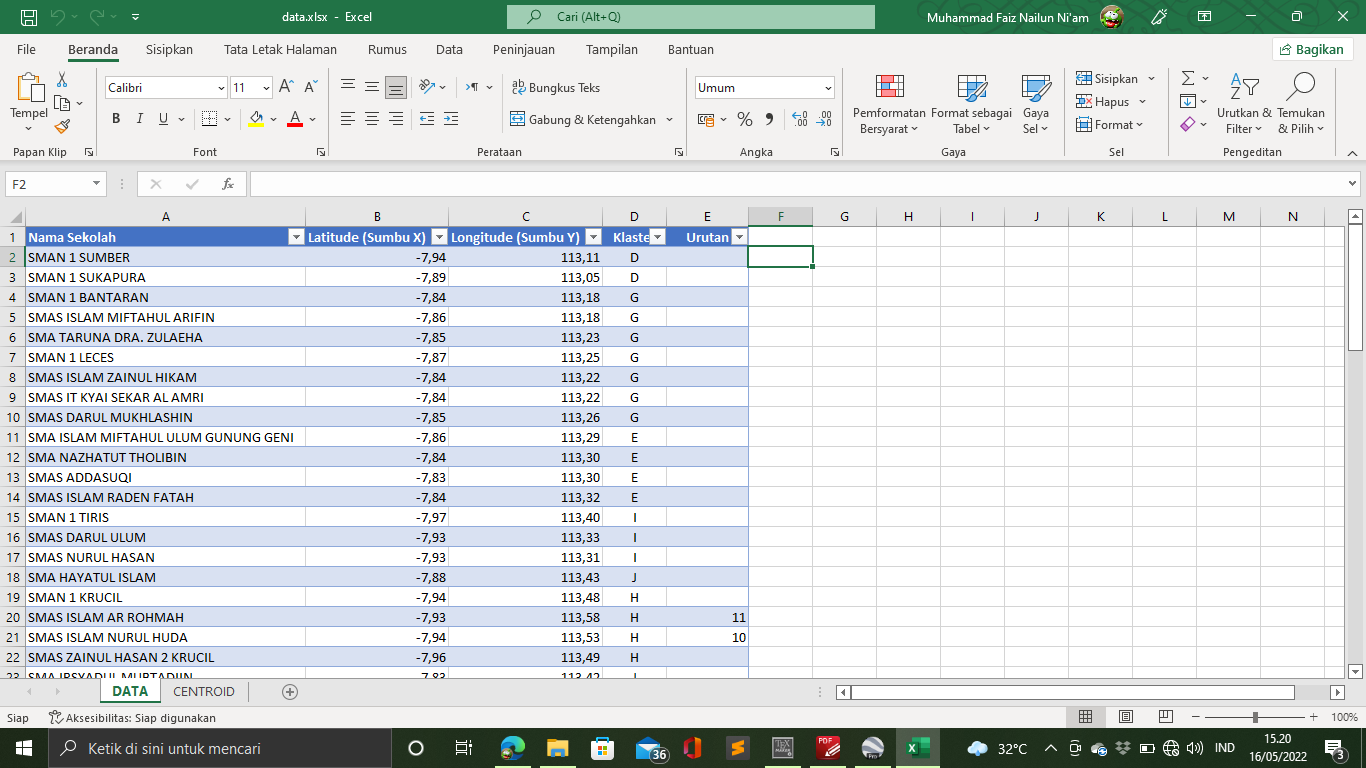
\includegraphics[width=0.8\textwidth]{ekspor excel.png}
  \caption{Mengekspor data dan menjadikannya ke format excel}
\end{figure}

\end{enumerate}

\subsection{Langkah-langkah Dalam Tahap Pengolahan Data}
\begin{enumerate}
    \item Menyiapkan data yang telah dikumpulkan sebelumnya.
    \item Selanjutnya menentukan jumlah klaster yaitu sebanyak $n$ klaster. Data yang telah dikumupulkan pada tahap ini akan dibagi menjadi beberapa klaster, metode yang digunakan algoritma \textit{k}-means.
    \item Langkah-langkah yang digunakan dalam metode \textit{k}-means adalah sebagai berikut
    \begin{enumerate}
        \item Memilih sebanyak $n$ \textit{centroid} secara acak, sesuai dengan berapa banyak salesman yang akan ditugaskan
        \item Menghitung jarak data ke \textit{centroid} dengan rumus \textit{euclidean distance}
        \begin{equation}
        d_{xy}=\sqrt{\sum_{i=1}^{n}(x_i-y_i)^{2}}
        \end{equation}
        \item Titik-titik lokasi yang tersebar merupakan klaster yang sama dengan titik \textit{centroid} paling dekat
        \item Perbarui \textit{centroid} tiap klaster yang dihasilkan dengan menghitung nilai koordinat rata-rata titik nilai pada masing-masing klaster.
        \item Iterasi dilakukan untuk generasi berikutnya sampai yaitu dengan kembali ke tahapan (b) sampai tidak ada perubahan klaster atau perubahan nilai \textit{centroid}
    \end{enumerate}
	
	\item Selanjutnya melakukan proses TSP pada setiap klaster yang telah dibagi, langkah-langkahnya adalah sebagai berikut.
	\begin{enumerate}
	    \item Membuat populasi awal secara random menggunakan data yang telah diklaster
	    \item Melakukan reproduksi dengan metode \textit{crosover} dengan peluang 0,95
	    \item Melakukan mutasi pada data dengan peluang 0,01
	    \item Selanjutnya seleksi dengan mode eliminasi
	    \item Menentukan nilai fitness agar mendapatkan solusi akhir yang optimaldengan rumus:
	    \begin{equation}
	    fitness=\frac{10000}{RMSE}
	    \end{equation}
	    \item Iterasi dilakukan dengan cara kembali ke tahapan b untuk generasi berikutnya sampai hasil yang dilakukan optimal atau mendekati optimal.
    \end{enumerate}
	\item Ketika proses diatas selesai dilakukan maka dihasilkanlah pembagian klaster dan rute terdekat tiap klaster menuju seluruh SMP di Kabupaten Probolinggo
	\item Mengevaluasi data yang dihasilkan
\end{enumerate}
%\section{Prosedur Penelitian dan Pengembangan}

Agar penulisan dalam penelitian yang diusulkan lebih terarah,
maka diperlukan sistematika penelitian.
Terkait hal tersebut,
sistematika penulisan dalam penelitian yang dilakukan nantinya adalah sebagai berikut.

\begin{enumerate}[label=]

	\item BAB I PENDAHULUAN 
	\begin{enumerate}[label=\Alph*.]
		\item Latar Belakang Masalah
		\item Rumusan Masalah
		\item Manfaat penelitian
		\item Tujuan Penelitian dan Pengembangan
		\item Batasan Masalah Penelitian
	\end{enumerate}

	\item BAB II KAJIAN PUSTAKA 
	\begin{enumerate}[label=\Alph*.]
		\item Penelitian relevan
		\item Dasar Teori
	\end{enumerate}

	\item BAB III KERANGKA TEORITIK DAN PENGEMBANGAN 
	\begin{enumerate}[label=\Alph*.]
		\item Model Penelitian dan Pengembangan
		\item Prosedur Penelitian dan Pengembangan
	\end{enumerate}

	\item BAB IV HASIL 
	\begin{enumerate}[label=\Alph*.]
		\item Penyajian Data Uji Coba
		\item Analisis Data
		\item Revisi Produk
	\end{enumerate}

	\item BAB V PENUTUP 
	\begin{enumerate}[label=\Alph*.]
		\item Kesimpulan
		\item Saran
	\end{enumerate}

\end{enumerate}


%penelitian akan mempu menghasilkan suatu produk yang memiliki nilai validasi tinggi, karena melalui serangkaian uji coba di lapangan dan divalidasi. Sistematika penelitian ini dibagi menjadi 4 tahap:
%
%\begin{enumerate}
%
%	\item Perencanaan
%	
%	Kegiatan yang dilakukan dalam tahap ini adalah sebagai berikut: penyusunan rancangan penelitian, penyiapan alat-alat penelitian, penetapan data penelitian, menyusun instrumen penelitian.
%	
%	\item Pelaksanaan
%	
%	Pada tahap ini peneliti selain pelaksana penelitian  juga mencari informasi data, yaitu membaca artikel penelitian sebelumnya yang berkaitan. Selain itu peneliti juga menyiapkan aplikasi yang akan digunakan untuk membantu perhitungan.
%	
%	\item Analisis Data
%	
%	Analisis data dilakukan setelah peneliti melakukan beberapa uji coba pada beberapa sampel data.
%	
%	\item Evaluasi Semua Data
%	
%	Data yang telah dianalisis kemudian dievaluasi sehingga diketahui bahwa metode ini merupakan metode yang efektif untuk menyelesaikan \textit{Multiple Traveling Salesman Problem} (MTSP).

%\end{enumerate}

\chapter{HASIL}
\section{Penyajian Data Uji Coba}

Pada penelitian ini dilakukan uji coba menggunakan data lokasi seluruh SMA di Kabupaten Probolinggo, dan dijalankan menggunakan python. Berikut adalah sajian data hasil uji coba.

\subsection{Pengambilan Data Lokasi}

Data yang digunakan adalah data koordinat lokasi yang diekspor melalui google earth. Pengujian Pengambilan data lokasi bertujuan untuk menunjukkan bahwa sistem 
mampu membaca input yang dimasukkan. Dapat dilihat pada Gambar \ref{fig:datalok} sebagian nama nama sekolah di kabupaten probolinggo beserta koordinat lokasinya. Visualisasi data dari koordinat-koordinat SMA di kabupaten probolinggo dapat dilihat pada Gambar \ref{fig:petasma}.

\begin{figure}[h!]
  \centering
  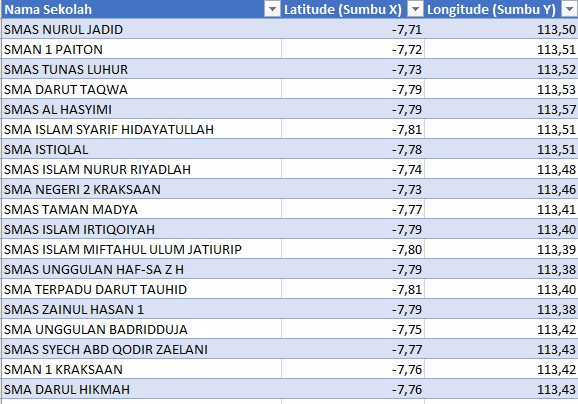
\includegraphics[width=0.8\textwidth]{data lokasi sekolah.png}
  \caption{Beberapa Data Lokasi Sekolah}
  \label{fig:datalok}
\end{figure}

\begin{figure}[h!]
  \centering
  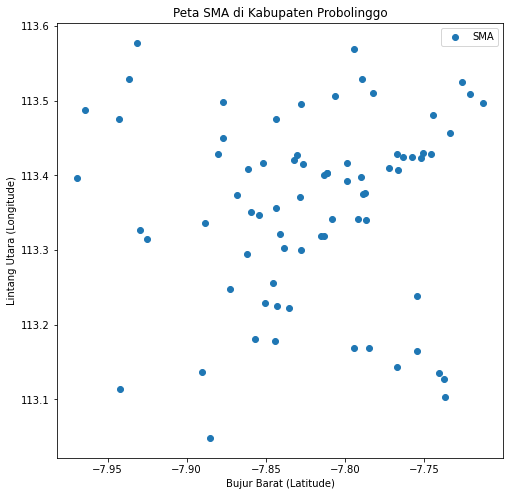
\includegraphics[width=0.5\textwidth]{peta sma.png}
  \caption{Visualisasi lokasi SMA di Kabupaten Probolinggo}
  \label{fig:petasma}
\end{figure}

Setelah mendapatkan lokasi yang akan diproses, selanjutnya adalah menentukan beberapa titik centroid secara random, dalam penelitian ini akan diambil 7 centroid secara random seperti pada Tabel \ref{tab:dasen} dan \ref{fig:visdasen}.

\begin{table}[H]
\centering
\begin{tabular}{cccll}
\cellcolor[HTML]{4472C4}{\color[HTML]{FFFFFF} \textbf{Nama   Centroid}} & \cellcolor[HTML]{4472C4}{\color[HTML]{FFFFFF} \textbf{Latitude (Sumbu X)}} & \cellcolor[HTML]{4472C4}{\color[HTML]{FFFFFF} \textbf{Longitude (Sumbu Y)}} &  &  \\
\cellcolor[HTML]{D9E1F2}A                                               & \cellcolor[HTML]{D9E1F2}-7,81                                              & \cellcolor[HTML]{D9E1F2}113,14                                              &  &  \\
B                                                                       & -7,77                                                                      & 113,51                                                                      &  &  \\
\cellcolor[HTML]{D9E1F2}C                                               & \cellcolor[HTML]{D9E1F2}-7,77                                              & \cellcolor[HTML]{D9E1F2}113,40                                              &  &  \\
D                                                                       & -7,88                                                                      & 113,35                                                                      &  &  \\
\cellcolor[HTML]{D9E1F2}E                                               & \cellcolor[HTML]{D9E1F2}-7,93                                              & \cellcolor[HTML]{D9E1F2}113,51                                              &  &  \\
F                                                                       & -7,83                                                                      & 113,27                                                                      &  &  \\
\cellcolor[HTML]{D9E1F2}G                                               & \cellcolor[HTML]{D9E1F2}-7,84                                              & \cellcolor[HTML]{D9E1F2}113,42                                              &  & 
\end{tabular}
\caption{Koordinat titik-titik centroid pada pembagian menjadi 8 klaster}
\label{tab:dasen}
\end{table}

\begin{figure}[h!]
	\centering
	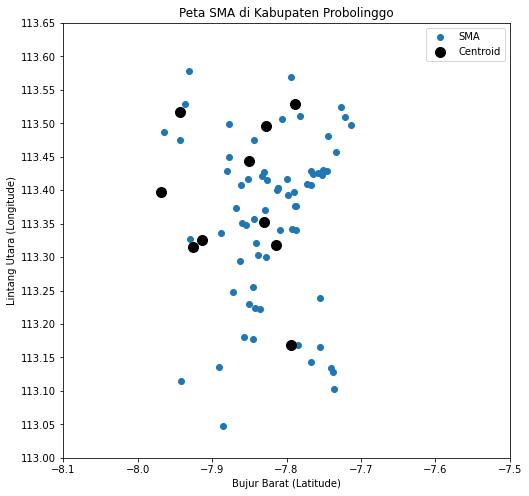
\includegraphics[width=0.5\textwidth]{titik centroid.png}
	\caption{Visualisasi Centroid}
	\label{fig:visdasen}
\end{figure}

\subsection{Proses Pengklasteran Data}

Pada tahap ini metode yang digunakan adalah metode $K-$means untuk mengklaster data. Langkah-langkah nya adalah sebagai berikut.

\begin{enumerate}
	\item Menentukan jumlah klaster, dalam hal ini yang digunakan adalah 7 klaster.
	\item Memilih titik-titik centroid sebanyak jumlah klaster seperti pada Tabel \ref{tab:dasen} dan \ref{fig:visdasen}
	\item \label{ulang3} Hitung jarak tiap titik sekolah yang ada dengan masing-masing \textit{centroid}. Penghitungan jarak menggunakan \textit{Euclidean Distance} pada persamaan (\ref{eq:euclidean3}.
	\item Kelompokan data ke dalam klaster yang memiliki jarak paling minimum.
	\item Setelah seluruh titik sekolah masuk ke dalam klaster-klaster, hitung \textit{centroid} yang baru dengan cara menghitung rata-rata titik sekolah yang ada di dalam klaster tersebut. Lakukan hal yang sama pada klaster yang lain.
	\item Jika terdapat perubahan klaster, maka ulangi langkah \ref{ulang3} hingga tidak ada perubahan anggota pada tiap klaster. Jika \textit{centroid} yang baru tidak berubah dari sebelumnya, maka proses berhenti, karena \textit{centroid} yang tidak berubah menyebabkan anggota klaster juga tidak berubah.
	
	\begin{equation}
	\left[ \left( x,y \right) ,\left( a,b \right)\right]=\sqrt{\left( x-a \right)^{2}+\left( y-b \right)^{2}}
	\label{eq:euclidean3}
	\end{equation}
	
	\item Setelah semua data terklasifikasi, selanjutnya adalah memperbarui titik-titik centroid dengan cara menghitung rata-rata tiap anggota klaster.
\end{enumerate}

\subsection{Proses TSP menggunakan Algoritma Genetika}

Setelah data terklaster seperti pada Gambar \ref{fig:hasilklas} selanjutnya adalah mencari rute terdekatnya menggunakan Algoritma Genetika

\begin{figure}[h!]
	\centering
	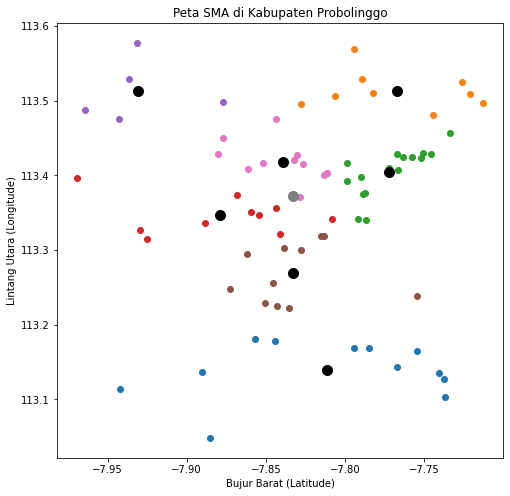
\includegraphics[width=0.5\textwidth]{hasil klaster.png}
	\caption{Visualisasi klaster sesuai warna}
	\label{fig:hasilklas}
\end{figure}

\begin{enumerate}
	\item Bangkitkan beberapa populasi awal berisi sejumlah kromosom yang di dalamnya terdapat urutan perjalanan menuju titik sekolah.
	\item \label{ulang4} Hitung nilai \textit{fitness} (total jarak) dari tiap kromosom.
	\item Menetapkan probabilitas \textit{crossover} ($p_c$) dalam hal ini yang digunakan adalah $p_c=0,95$. Bangkitkan bilangan random (0,0000 sampai 1,0000) pada setiap kromosom, kromosom dengan bilangan random kurang dari $p_c$ maka akan dilakukan \textit{crossover}. Jika kromosom hasil \textit{crossover} memiliki \textit{fitness} yang lebih baik  dari kromosom awal, maka kromosom awal digantikan oleh kromosom hasil \textit{crossover}.
	\item Menetapkan probabilitas mutasi ($p_m$), dalam hal ini digunakan $p_m=0,1$. Bangkitakan bilangan random (0,0000 sampai 1,0000) pada setiap kromosom, kromosom yang memiliki bilangan random kuran dari $p_m$ maka akan dilakukan mutasi. Jika kromosom hasil mutasi memiliki \textit{fitness} yang lebih baik dari kromosom awal, maka kromosom awal digantikan oleh kromosom hasil mutasi.
	\item Jika hasil kurang optimal, iterasi dilakukan dengan cara kembali ke tahapan (\ref{ulang4}) untuk generasi berikutnya sampai hasil yang dilakukan optimal atau mendekati optimal.
\end{enumerate}

\subsection{Hasil dari proses \textbf{$k$}-means dan Algoritma Genetika}

Dari serangkaian proses di atas, menghasilkan beberapa rute optimal yang dapat dilalui seperti pada Gambar \ref{fig:vishasilmtsp}. Rute-rute yang dihasilkan telah diurutkan sebelumnya dan telah diekspor ke bentuk spreadsheet sehingga mempermudah pengguna dalam membaca data seperti pada Tabel \ref{tab:datahasil} merupakan urutan perjalanan pada klaster A.

\begin{figure}[h!]
	\centering
	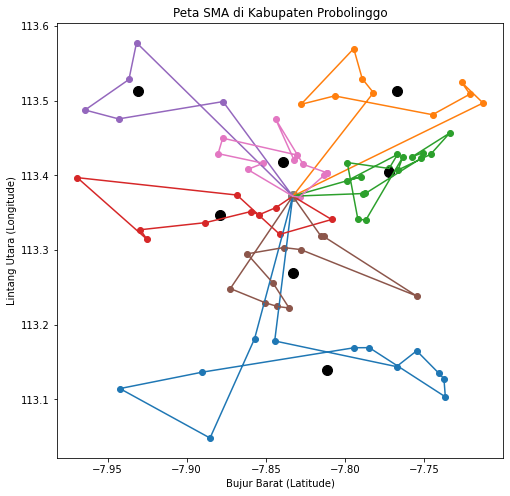
\includegraphics[width=0.5\textwidth]{hasil mtsp.png}
	\caption{Visualisasi hasil pembagian klaster dan rute yang dapat dilalui}
	\label{fig:vishasilmtsp}
\end{figure}

\begin{table}[h!]
\begin{adjustbox}{width=\columnwidth,center}
\begin{tabular}{lllcl}
\rowcolor[HTML]{4472C4} 
\multicolumn{1}{c}{\cellcolor[HTML]{4472C4}{\color[HTML]{FFFFFF} \textbf{Nama   Sekolah}}} & \multicolumn{1}{c}{\cellcolor[HTML]{4472C4}{\color[HTML]{FFFFFF} \textbf{Latitude (Sumbu X)}}} & \multicolumn{1}{c}{\cellcolor[HTML]{4472C4}{\color[HTML]{FFFFFF} \textbf{Longitude (Sumbu Y)}}} & {\color[HTML]{FFFFFF} \textbf{Klaster}} & \multicolumn{1}{c}{\cellcolor[HTML]{4472C4}{\color[HTML]{FFFFFF} \textbf{Urutan}}} \\
\rowcolor[HTML]{D9E1F2} 
SMAS ISLAM MIFTAHUL ARIFIN                                                                 & -7,86                                                                                          & 113,18                                                                                          & A                                       & 0                                                                                  \\
SMAN   1 SUKAPURA                                                                          & -7,89                                                                                          & 113,05                                                                                          & A                                       & 1                                                                                  \\
\rowcolor[HTML]{D9E1F2} 
SMAN 1 SUMBER                                                                              & -7,94                                                                                          & 113,11                                                                                          & A                                       & 2                                                                                  \\
SMA   NEGERI 1 KURIPAN                                                                     & -7,89                                                                                          & 113,14                                                                                          & A                                       & 3                                                                                  \\
\rowcolor[HTML]{D9E1F2} 
SMAS ISLAM SUMBERASIH                                                                      & -7,79                                                                                          & 113,17                                                                                          & A                                       & 4                                                                                  \\
SMAS   WALI SONGO                                                                          & -7,78                                                                                          & 113,17                                                                                          & A                                       & 5                                                                                  \\
\rowcolor[HTML]{D9E1F2} 
SMAN 1 TONGAS                                                                              & -7,74                                                                                          & 113,10                                                                                          & A                                       & 6                                                                                  \\
SMAS   ISLAM TAJUNG SARI                                                                   & -7,74                                                                                          & 113,13                                                                                          & A                                       & 7                                                                                  \\
\rowcolor[HTML]{D9E1F2} 
SMA NEGERI 1 SUMBERASIH                                                                    & -7,74                                                                                          & 113,13                                                                                          & A                                       & 8                                                                                  \\
SMAS   ASSUBHAN                                                                            & -7,75                                                                                          & 113,16                                                                                          & A                                       & 9                                                                                  \\
\rowcolor[HTML]{D9E1F2} 
SMAS DARUL AKHLAQ                                                                          & -7,77                                                                                          & 113,14                                                                                          & A                                       & 10                                                                                 \\
SMAN   1 BANTARAN                                                                          & -7,84                                                                                          & 113,18                                                                                          & A                                       & 11                                                                                
\end{tabular}
\end{adjustbox}
\caption{Urutan perjalanan pada klaster A}
\label{tab:datahasil}
\end{table}
\section{Analisis Data}
\section{Revisi Produk}

\chapter{PENUTUP}
\section{Kesimpulan}
\section{Saran}
% Daftar Pustaka
\newpage
\bibliographystyle{apalike}
\bibliography{library}

\newpage
\thispagestyle{empty}
\addcontentsline{toc}{chapter}{LAMPIRAN}

\section*{Lampiran 1 Daftar Hadir Peserta}

%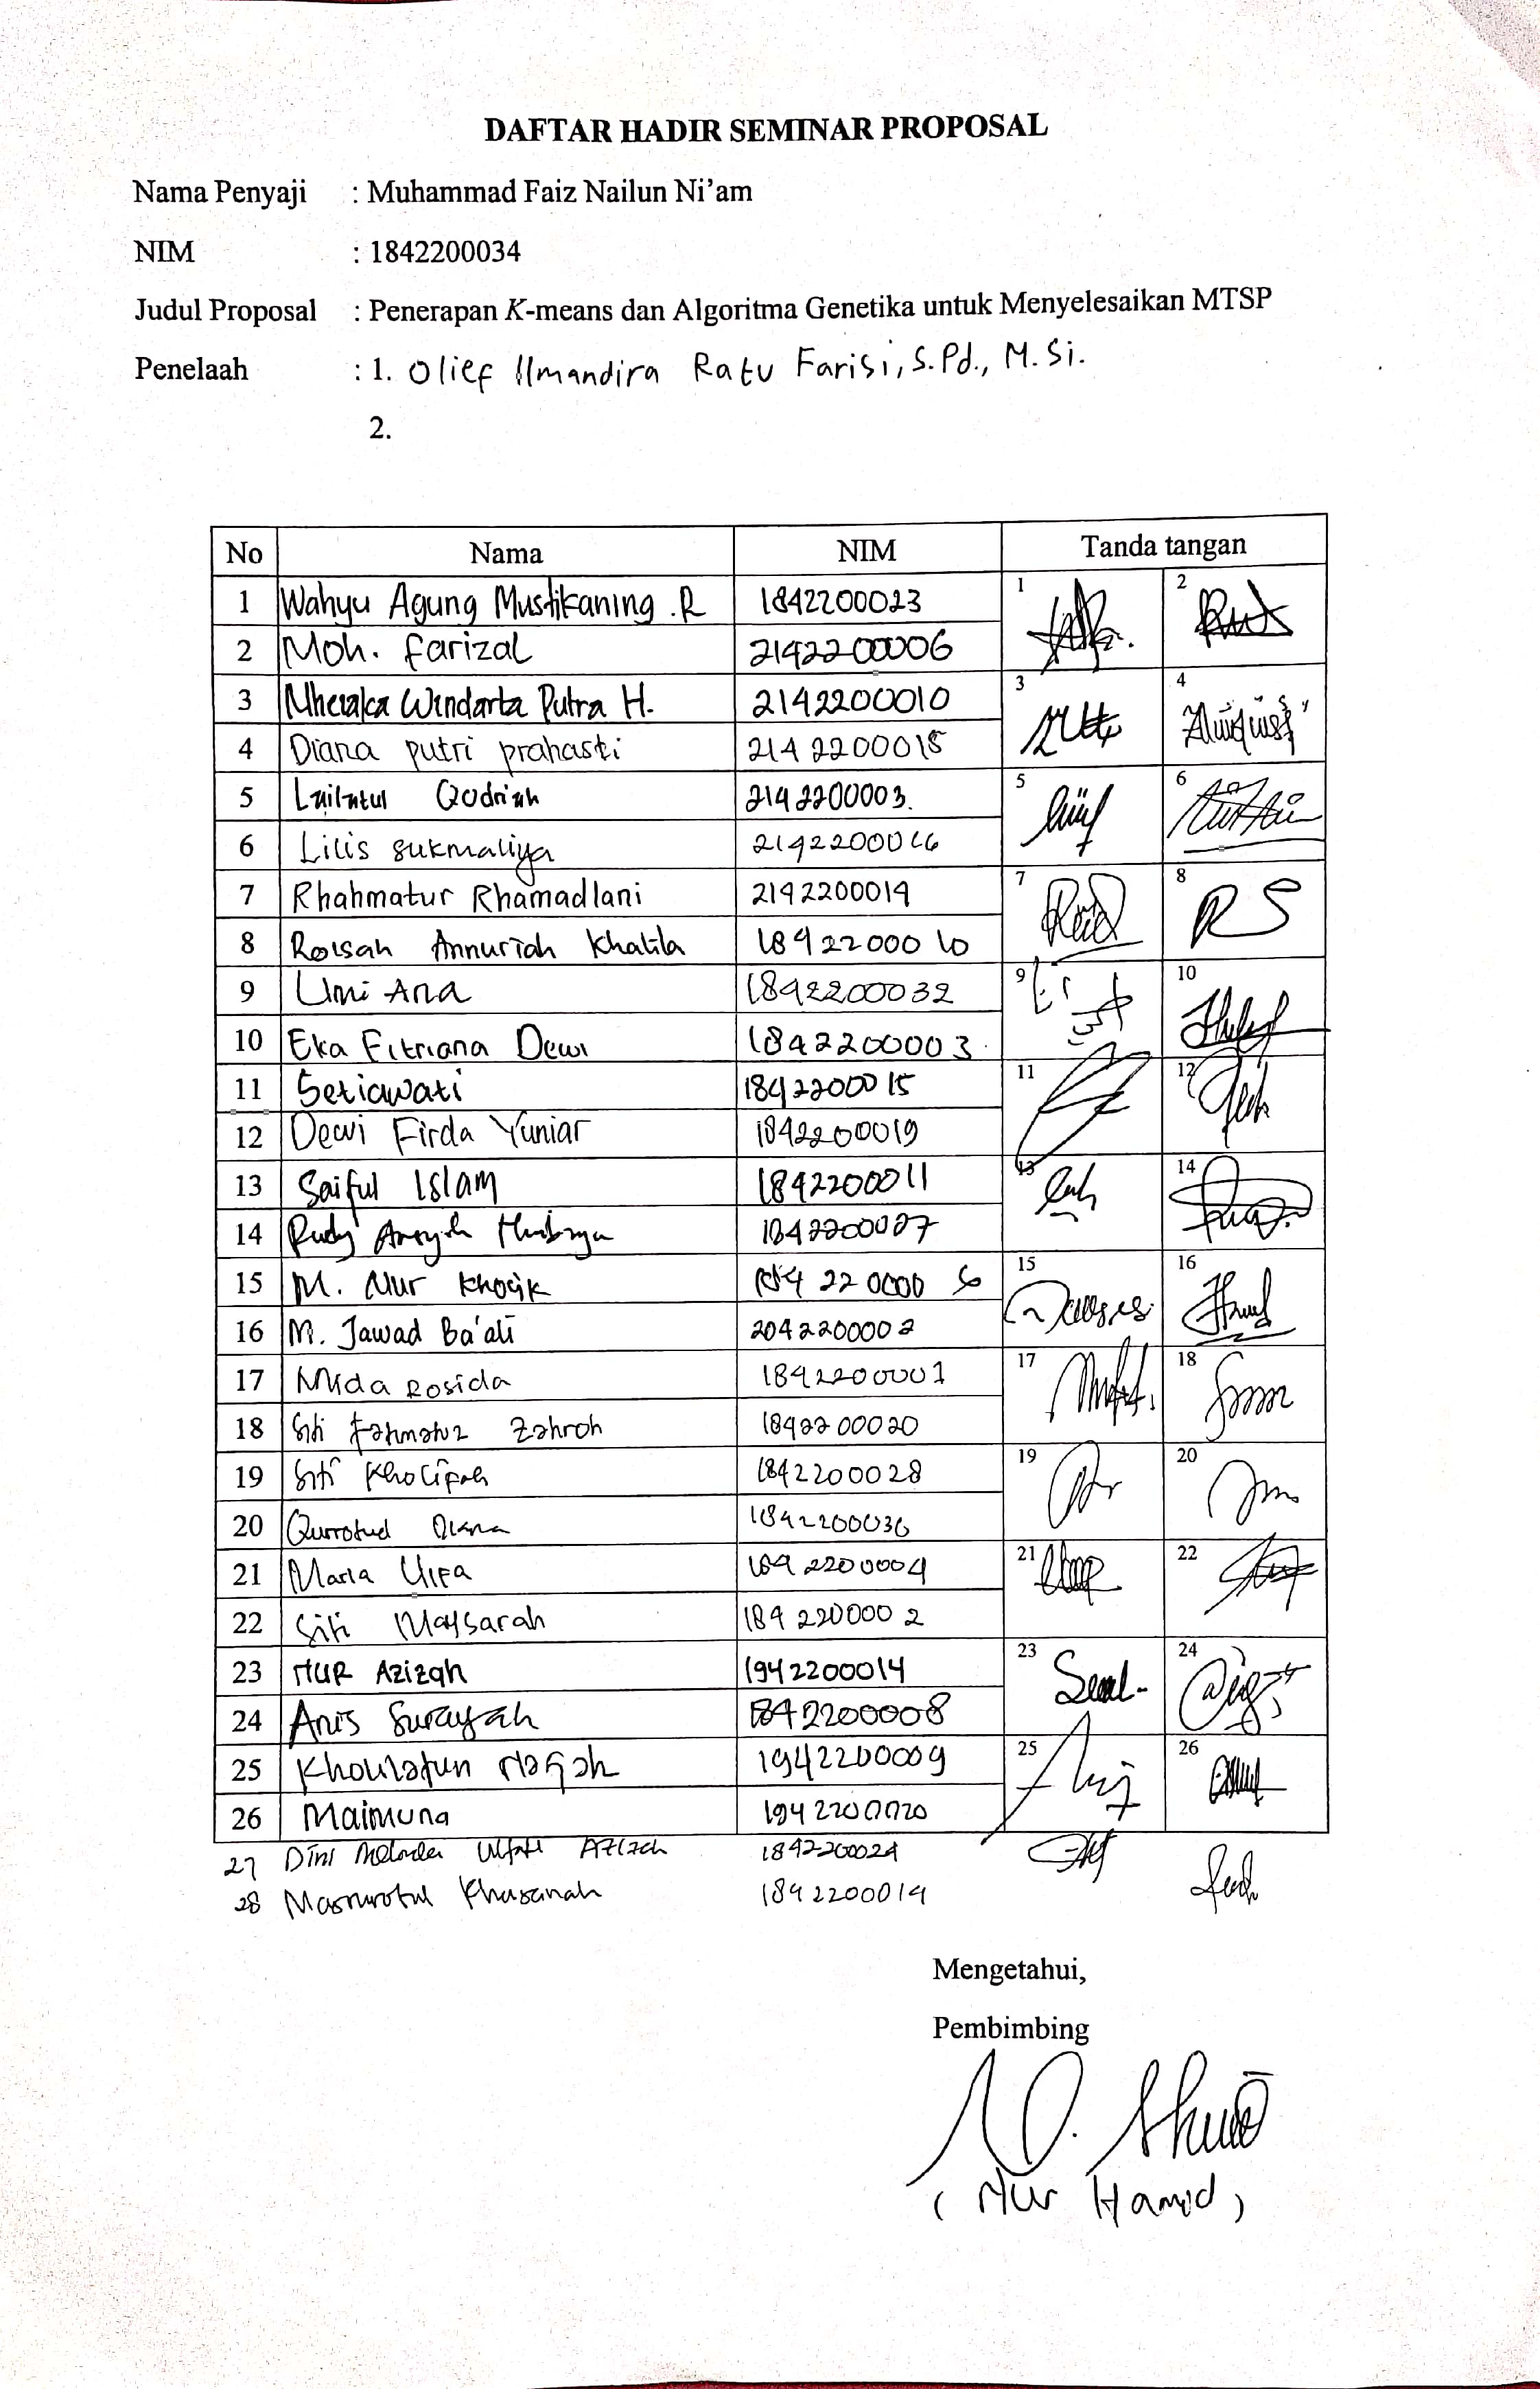
\includegraphics[height=21cm]{daftar_hadir_1.jpg} 

%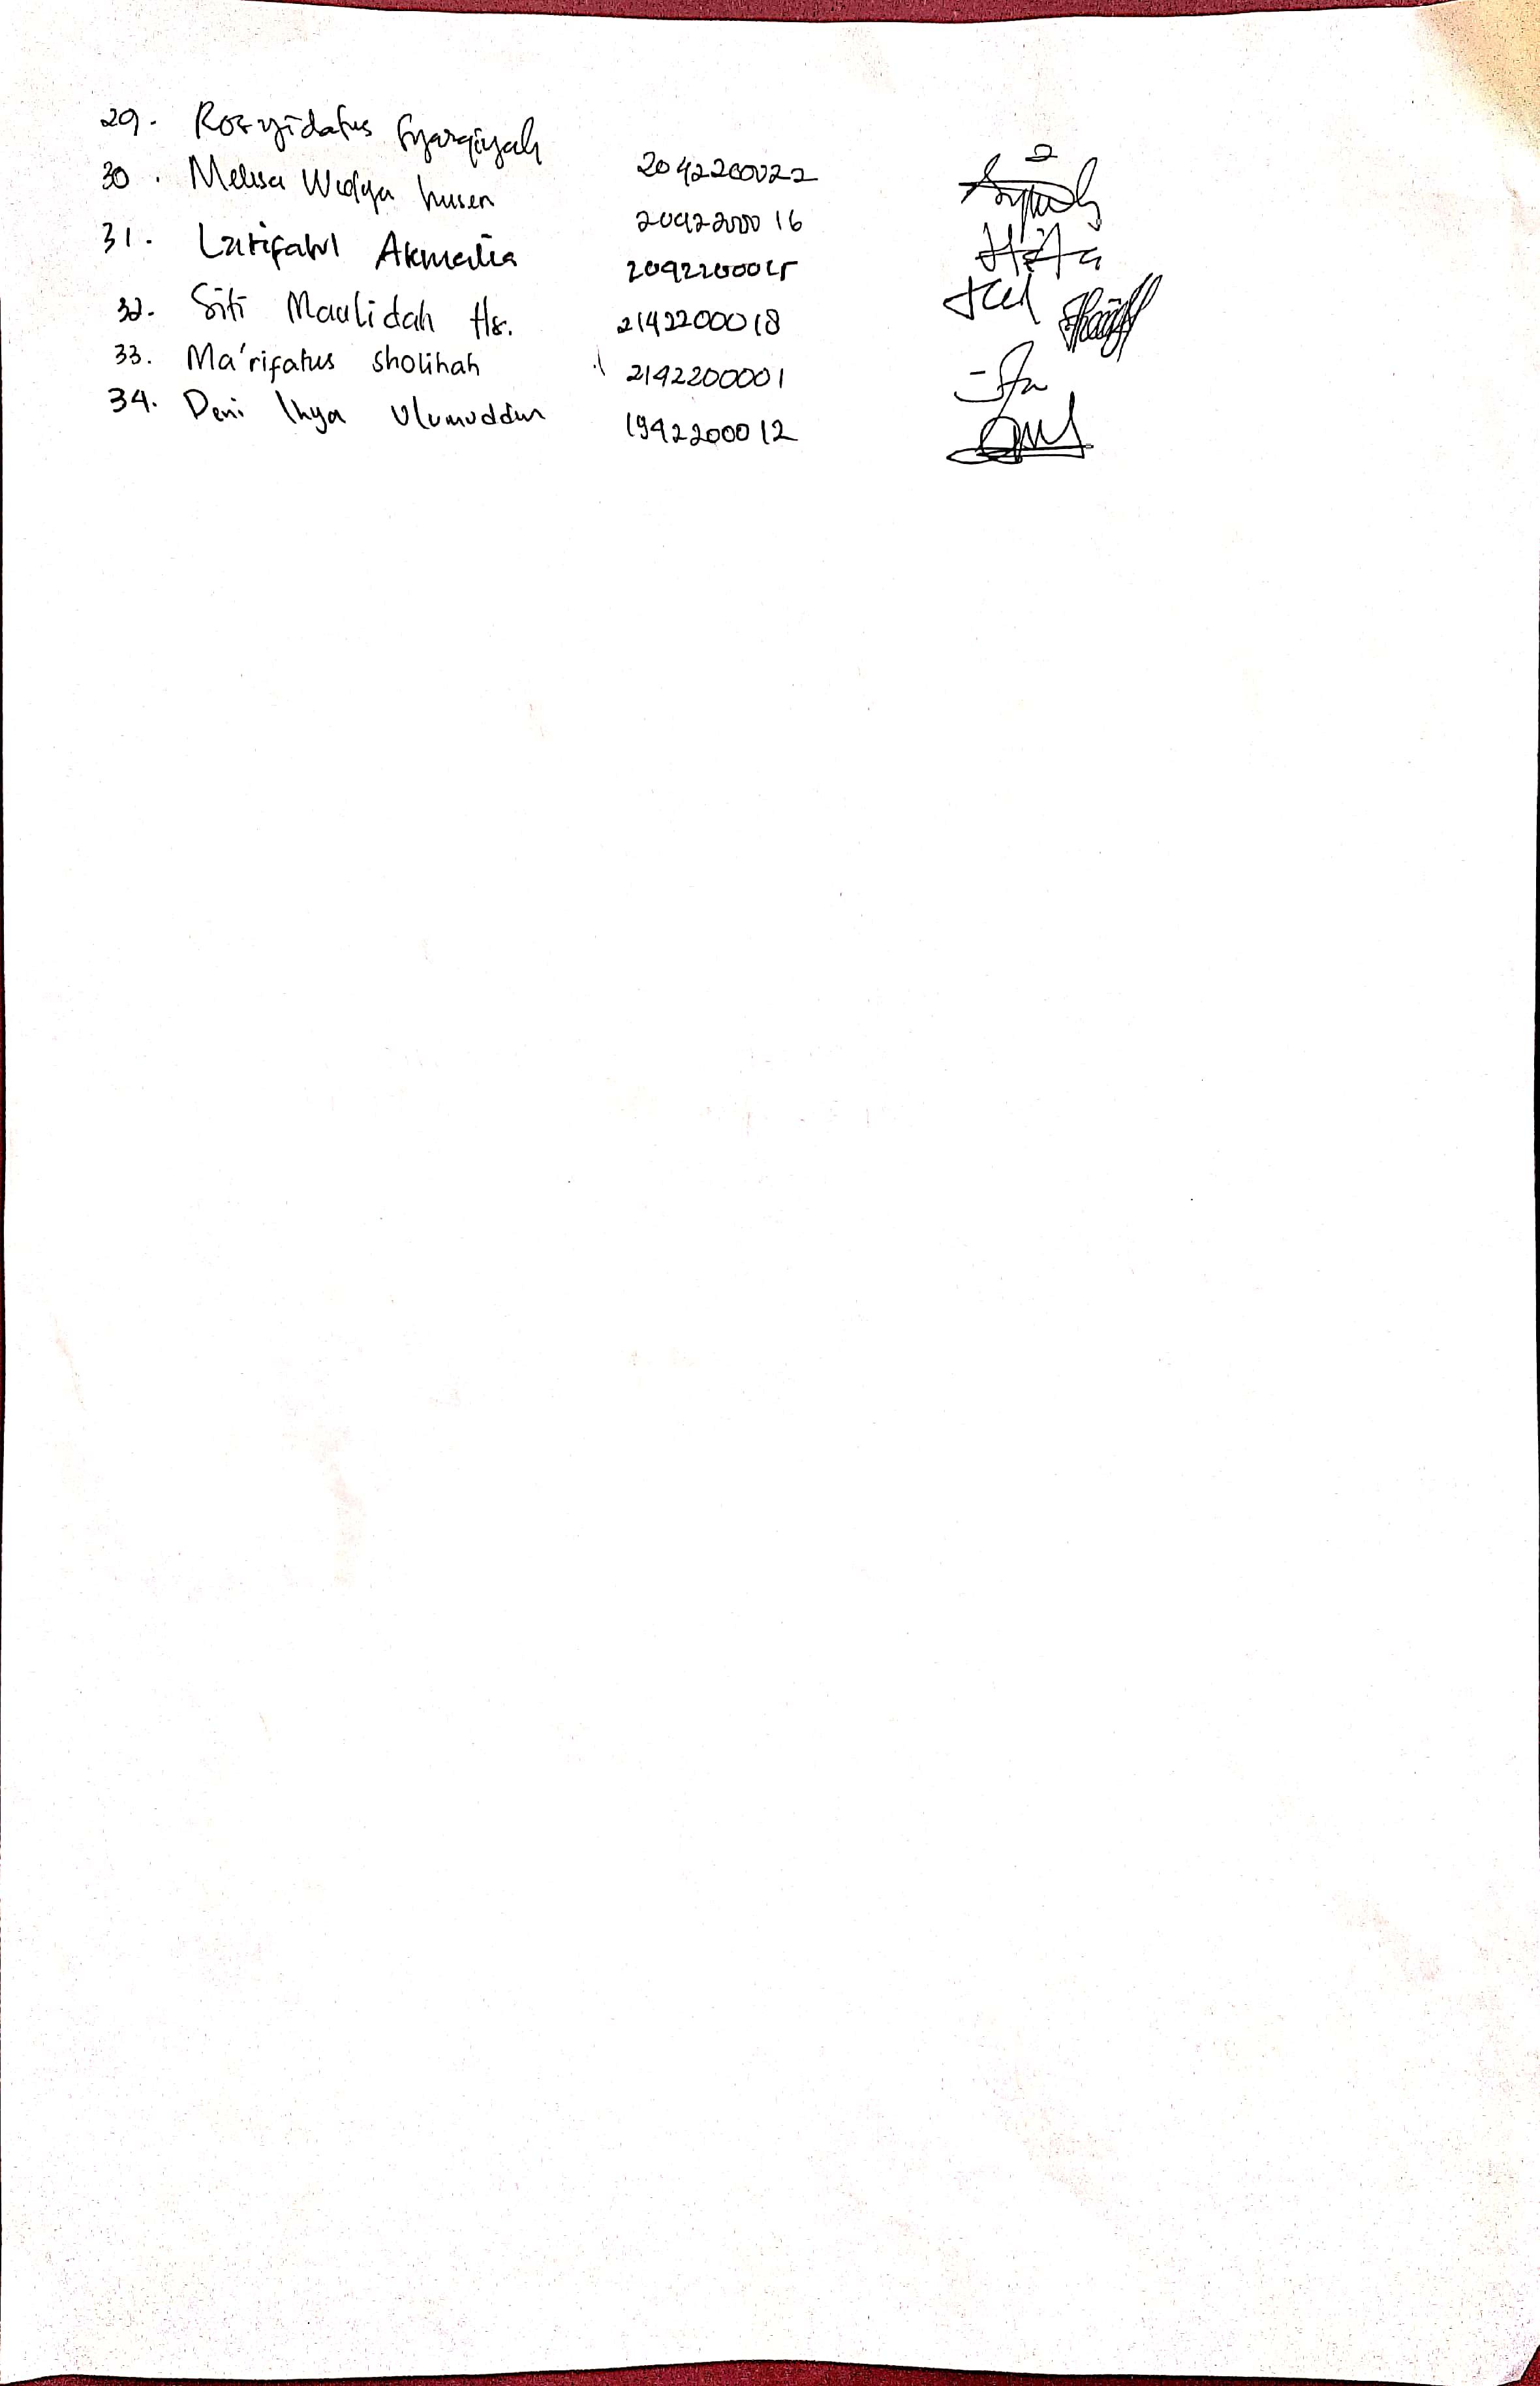
\includegraphics[height=21cm]{daftar_hadir_2.jpg}

\newpage
\thispagestyle{empty}
\section*{Lampiran 2 Instrumen Penelitian}

%\begin{enumerate}
%\item Jupyter Notebook

%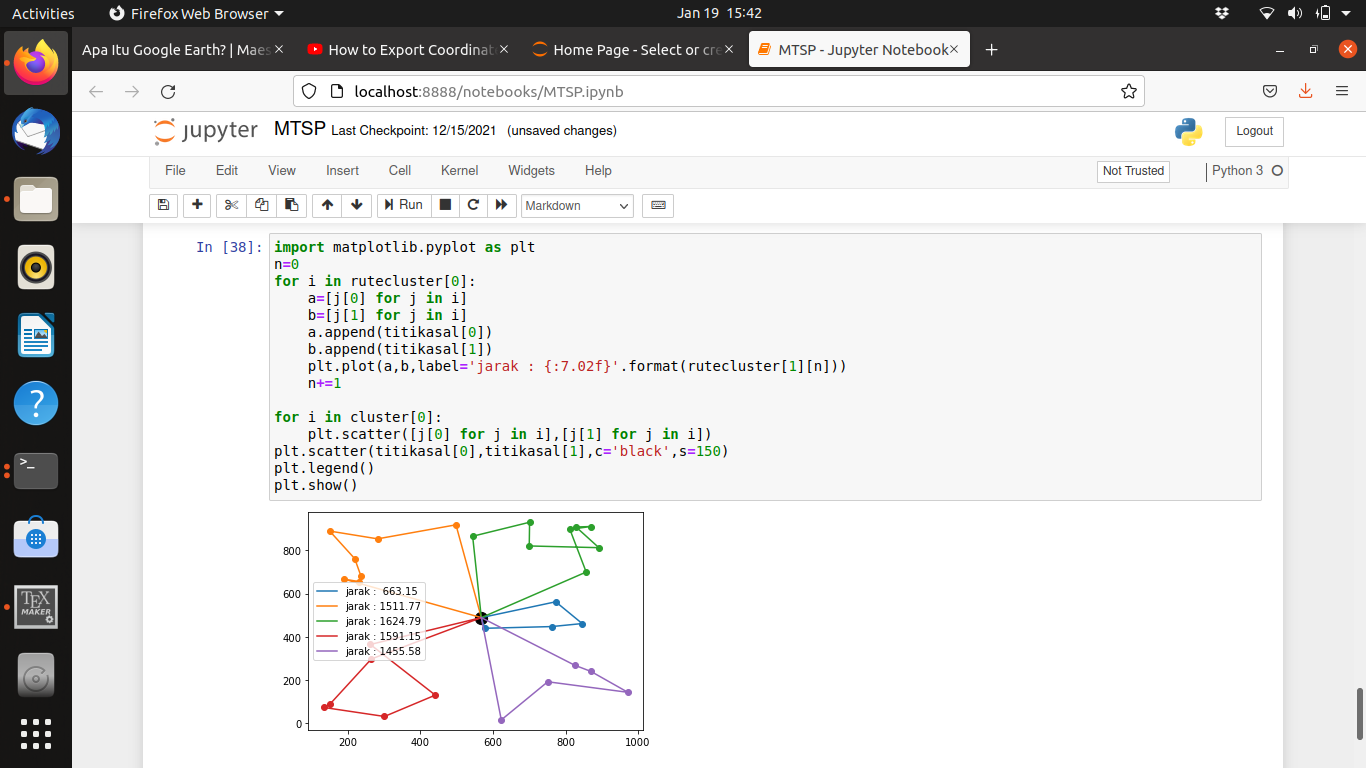
\includegraphics[width=13cm]{instrumen2.png}

%\item Google Earth

%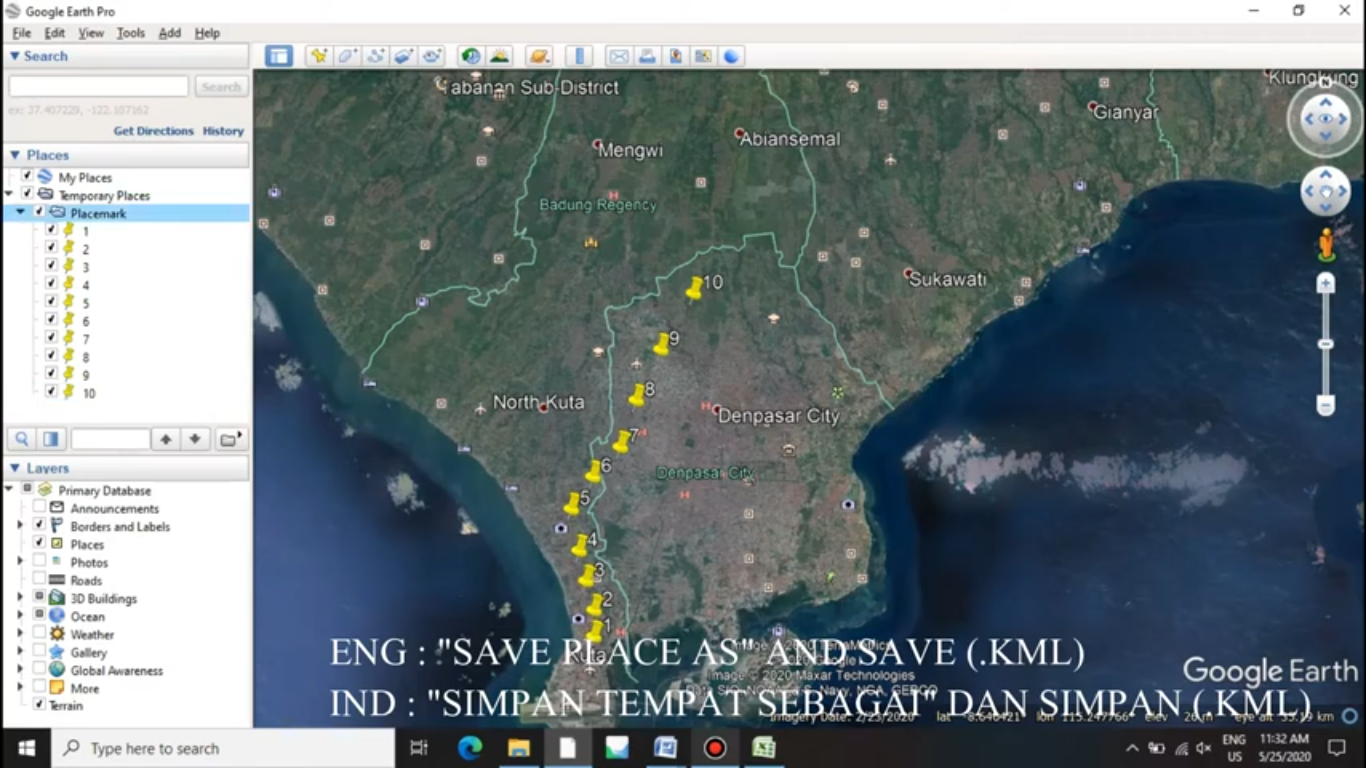
\includegraphics[width=13cm]{instrumen1.png}

%\end{enumerate}

\newpage
%\addcontentsline{toc}{chapter}{RIWAYAT HIDUP}
\chapter*{RIWAYAT HIDUP}

\noindent
\begin{wrapfigure}{l}{3cm}

\includegraphics[width=3cm, height=4cm]{Gambar/pas foto.jpg} 
\end{wrapfigure}

Muhammad Faiz Nailun Ni'am, dilahirkan di Kabupaten Bondowoso tepatnya di Desa Tegal Mijin pada hari Rabu tanggal 12 Januari 2000. Anak pertama dari tiga bersaudara, terlahir dari pasangan Abdul Hadi dan Hosni. Peneliti menyelesaikan pendidikan Sekolah Dasar di SD Negeri Tegal Mijin 1 di Kecamatan Grujugan Kabupaten Bondowoso pada tahun 2012. Pada tahun itu juga peneliti melanjutkan Pendidikan di SMP Negeri 1 Jambesari Darussholah Kecamatan Jambesari Kabupaten Bondowoso dan selesai pada tahun 2015, kemudian melanjutkan Sekolah Menengah Atas di pesantren yaitu SMA Nurul Jadid yang berada di Pondok Pesantren Nurul Jadid Kecamatan Paiton Kabupaten Probolinggo dan selesai pada tahun 2018. Pada saat SMA peneliti mendapat berpengalaman meraih juara 2 di bidang matematika pada Kompetisi Sains Nalaria Realistik (KSNR) tingkat kabupaten pada tahun 2015 serta juara 2 di bidang informatika pada Olimpiade Sains Nasional (OSN) tingkat kabupaten pada tahun 2016.

Pada tahun 2018 peneliti melanjutkan pendidikan di perguruan tinggi swasta, tepatnya di Universitas Nurul Jadid Program Studi Pendidikan Matematika. Pengalaman saat di Universitas peneliti pernah menjadi Sekretaris Himaprodi Pendidikan Matematika Masa Bakti 2020/2021, anggota dan tenaga pengajar Bimbingan Belajar PCC Math (Personal Computer Community Of Mathematic). Peneliti pernah menjadi asisten dosen mata kuliah Pengantar Dasar Komputer Pada Februari sampai Juni 2021 di Pendidikan Matematika. Pada maret sampai april 2022 Peneliti menjadi pembimbing dalam pengabdian bersama dosen dalam pembinaan KSN Informatika Tahun 2022 di SMA Tunas Luhur Paiton Probolinggo. Selain itu peneliti juga pernah berprofesi sebagai asisten guru di MA Nurul Jadid Kecamatan Paiton Kabupaten Probolinggo. 
\end{document}